\documentclass[whitelogo]{TUD-report2020}

\usepackage{changes}
\definechangesauthor[name=Ojas, color=tudelft-orange]{1}
\usepackage[utf8]{inputenc} % allow utf-8 input
\usepackage[T1]{fontenc}    % use 8-bit T1 fonts
\usepackage{csquotes}
\usepackage{times}
\usepackage{epsfig}
\usepackage{graphicx}
\usepackage{svg}
\usepackage{unicode-math}
\usepackage{amsmath}
\usepackage{amssymb}
\usepackage{booktabs}
% Include other packages here, before hyperref.
\usepackage{stfloats}
\usepackage{bm}
\usepackage{flushend}
\usepackage{lipsum}

\usepackage[ruled,vlined]{algorithm2e}
% \SetAlFnt{\small}
% \SetAlCapFnt{\small}
\usepackage{enumitem}
\usepackage{arydshln}
\usepackage{colortbl}
\usepackage{tabularx}
\usepackage{ragged2e}
\usepackage{array}
\usepackage{threeparttablex}
\usepackage{makecell}
\usepackage{overpic}
\usepackage{pifont}
\newcommand{\cmark}{\ding{51}}%
\newcommand{\xmark}{\ding{55}}%
\usepackage{color}
\usepackage{url}
\usepackage[scr=boondoxo]{mathalpha}
% \usepackage{mathtools}

\usepackage{adjustbox}
\usepackage{setspace}
\usepackage{xargs}
% \usepackage[pdftex,dvipsnames]{xcolor}

\usepackage{caption}
\usepackage{subcaption}

\usepackage{url}            % simple URL typesetting
\usepackage{amsfonts}       % blackboard math symbols
\usepackage{xfrac}          % compact symbols for 1/2, etc.
\usepackage{microtype}      % microtypography

\usepackage{tikz}
\usepackage{comment}

\usepackage[skip=10pt plus1pt, indent=30pt]{parskip}
\usepackage{pdfpages}
\usepackage{import}
\usepackage{pgffor}

\usepackage{hyperref}
\usepackage[nameinlink]{cleveref}
\definecolor{darkred}{rgb}{0.5,0,0}
\definecolor{darkgreen}{rgb}{0,0.5,0}
\definecolor{darkblue}{rgb}{0,0,0.5}
\definecolor{gray}{rgb}{0.35,0.35,0.35}
\hypersetup{ colorlinks,
linkcolor=darkblue,
filecolor=darkblue,
urlcolor=darkblue,
citecolor=tudelft-lavendel}

\usepackage[citestyle=authoryear-comp, sorting=ynt, backref=true]{biblatex}
\addbibresource{report.bib}

\begin{document}

%% Use Roman numerals for the page numbers of the title pages and table of
%% contents.
\frontmatter

%% Uncomment following 19 lines for a cover with a picture on the lower half only
%\title[tudelft-white]{Title}
%\subtitle[tudelft-cyan]{Optional subtitle}
%\author[tudelft-white]{J.\ Random Author}
%\affiliation{Technische Universiteit Delft}
%\coverimage{cover.jpg}
%\titleoffsetx{10cm}
%\titleoffsety{10cm}
%\afiloffsetx{1cm}
%\afiloffsety{18cm}
%\covertext[tudelft-white]{
%    \textbf{Cover Text} \\
%    possibly \\
%    spanning 
%    multiple 
%    lines
%    \vfill
%    ISBN 000-00-0000-000-0
%}
%\makecover

%% Uncomment following 16 lines for a cover with a picture on the lower half only
\title[tudelft-white]{Title}
\subtitle[tudelft-white]{Optional subtitle}
\author[tudelft-white]{Ojas Kishorkumar Shirekar}
\affiliation{Technische Universiteit Delft}
\coverimage{neural.jpg}
% \covertext[tudelft-white]{
%     \textbf{Cover Text} \\
%     possibly \\
%     spanning 
%     multiple 
%     lines
%     \vfill
%     ISBN 000-00-0000-000-0
% }
\setpagecolor{tudelft-black}
\makecover[split]


%% Include an optional title page.
\begin{titlepage}


\begin{center}

%% Insert the TU Delft logo at the bottom of the page.

%% Print the title in cyan.
{\makeatletter
\largetitlestyle\fontsize{64}{94}\selectfont\@title
%\largetitlestyle\color{tudelft-cyan}\Huge\@title
\makeatother}

%% Print the optional subtitle in black.
{\makeatletter
\ifx\@subtitle\undefined\else
    \bigskip
   {\tudsffamily\fontsize{22}{32}\selectfont\@subtitle}    
    %\titlefont\titleshape\LARGE\@subtitle
\fi
\makeatother}

\bigskip
\bigskip

by
%door

\bigskip
\bigskip

%% Print the name of the author.
{\makeatletter
%\largetitlefont\Large\bfseries\@author
\largetitlestyle\fontsize{26}{26}\selectfont\@author
\makeatother}

\bigskip
\bigskip

to obtain the degree of Master of Science
%ter verkrijging van de graad van Master of Science

at the Delft University of Technology,
%aan de Technische Universiteit Delft,

to be defended publicly on Wednesday August 31, 2022 at 14:30.
%in het openbaar de verdedigen op dinsdag 1 januari om 10:00 uur.

\vfill

\begin{tabular}{lll}
    Student number: & 5225493 \\
    Project duration: & \multicolumn{2}{l}{July 1, 2021 -- July 31, 2022} \\
    Thesis committee: & Dr.\ H.\ Jamali-Rad, & TU Delft and Shell, Daily supervisor \\
        & Dr.\ ir.\ J.\ van Gemert, & TU Delft, Advisor \\
        & Dr.\ E.\ Isufi, & TU Delft, External committee member
\end{tabular}
%% Only include the following lines if confidentiality is applicable.

\bigskip
\bigskip
% \emph{This thesis is confidential and cannot be made public until December 31, 2013.}
%\emph{Op dit verslag is geheimhouding van toepassing tot en met 31 december 2013.}

\bigskip
\bigskip
An electronic version of this thesis is available at \url{http://repository.tudelft.nl/}.
%\\[1cm]

%\centering{
\includegraphics{cover/logo_black}}


\end{center}

\begin{tikzpicture}[remember picture, overlay]
    \node at (current page.south)[anchor=south,inner sep=0pt]{
        
\includegraphics{cover/logo_black}
    };
\end{tikzpicture}

\end{titlepage}



\chapter*{Preface}
\setheader{Preface}

This report, along with the two scientific articles present in it, is the culmination of the work I did for my Master's thesis. First, I would like to thank my supervisor and mentor, Dr.~Hadi Jamali-Rad, for the constant guidance and support. Much of this work would not have come to fruition if not for Hadi's drive and impeccable attention to detail. Not only has Hadi taught me whatever I know about the art of research, but he also imparted valuable life lessons that will always stay with me.

I would like to express my gratitude to my parents, brother and girlfriend. Without whose support, understanding and encouragement, I would not have the privilege of being able to pursue my interests or write this report while sitting in Delft.

Finally, I would like to thank the thesis committee chair, Dr.~Jan van Gemert, for his fantastic and exciting Deep Learning and Computer Vision classes that I always looked forward to attending. I would also like to thank Dr.~Elvin Isufi for their time and interest in my work, particularly during a busy and sweltering summer.

I am glad to have met some of the brightest people I know in Delft, and some have become my close friends. I cherish all my moments with them, especially the time spent in building 28. Thank you for making this journey colourful.

Working through my thesis, I have realised that my passion for computer science and research remains stronger than ever before.

This report has been structured to first show the two scientific articles containing the motivation, explanations, methods developed, and experimental results. The chapters following the articles present the fundamental concepts that have made this work a reality. The report has been designed to be as self-contained as possible.

\begin{flushright}
{\makeatletter\itshape
    \@author \\
    Delft, August 2022
\makeatother}
\end{flushright}

\tableofcontents

%% Use Arabic numerals for the page numbers of the chapters.
\mainmatter

\chapter{Scientific Article 1}
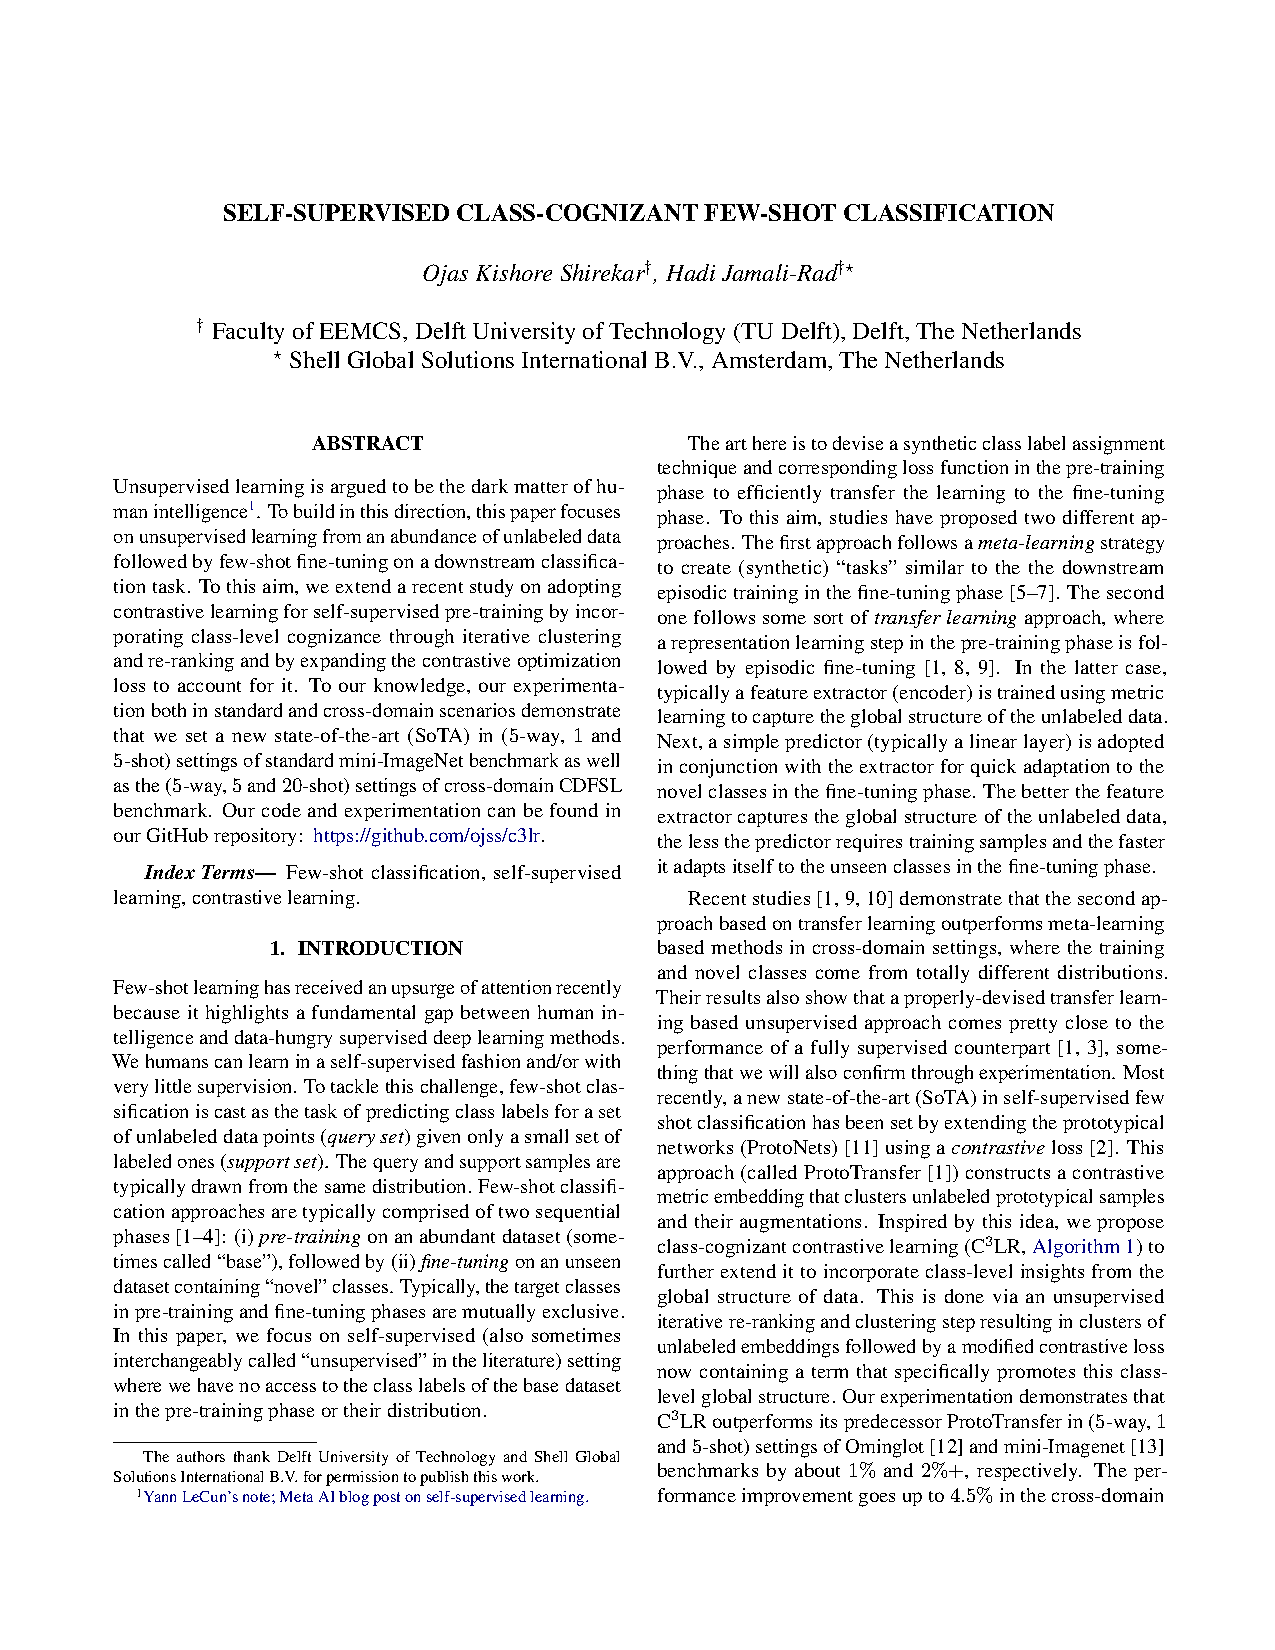
\includepdf[pages=-, pagecommand={}]{chapters/articles/c3lr/ICIP_C3LR_final.pdf}

\newcommand{\mA}{\symbfit{A}}
\newcommand{\mB}{\symbfit{B}}
\def\mI{\symbfit{I}}
\def\va{{\symbfit{a}}}
\def\ve{{\symbfit{e}}}
\def\vx{{\symbfit{x}}}
\def\vy{{\symbfit{y}}}
\def\mJ{{\symbfit{J}}}
\def\mH{{\symbfit{H}}}
\def\mX{{\symbfit{X}}}
% Random var
\def\ra{{\textnormal{a}}}
\def\rva{{\symbf{a}}}
\def\rmA{\symbf{\textnormal{A}}}
% Tensor

\newcommand{\tens}[1]{\symbfit{\mathsfit{#1}}}
\newcommand{\etens}[1]{\mathsfit{#1}}
\def\tA{{\tens{A}}}
\def\tX{{\tens{X}}}

\newcommand{\R}{\mathbb{R}}
\def\sS{{\mathbb{S}}}

\def\eva{{a}}
\def\emA{{A}}
\def\erva{{\textnormal{a}}}
\def\etA{{\etens{A}}}

% Sets
\def\sA{{\mathbb{A}}}
\def\sB{{\mathbb{B}}}
\def\sC{{\mathbb{C}}}
\def\sD{{\mathbb{D}}}

% Graph
\def\gA{{\mathcal{A}}}
\def\gB{{\mathcal{B}}}
\def\gC{{\mathcal{C}}}
\def\gD{{\mathcal{D}}}
\def\gE{{\mathcal{E}}}
\def\gF{{\mathcal{F}}}
\def\gG{{\mathcal{G}}}


\newcommand{\pdata}{p_{\rm{data}}}
% The empirical distribution defined by the training set
\newcommand{\ptrain}{\hat{p}_{\rm{data}}}


\makenomenclature
% \renewcommand{\nomname}{\makebox[\linewidth]{Notation}}
\renewcommand{\nomname}{Notation}
\renewcommand{\nomlabel}[1]{\hfil #1\hfil}

%% This code creates the groups
% -----------------------------------------
\renewcommand\nomgroup[1]{%
  \item[\bfseries
  \ifstrequal{#1}{A}{\centerline{Numbers and Arrays}}{%
  \ifstrequal{#1}{B}{\centerline{Linear Algebra Operations}}{%
  \ifstrequal{#1}{C}{\centerline{Indexing}}{%
  \ifstrequal{#1}{D}{\centerline{Calculus}}{%
  \ifstrequal{#1}{E}{\centerline{Sets and Graphs}}{%
  \ifstrequal{#1}{F}{\centerline{Probability and Information Theory}}{%
  \ifstrequal{#1}{G}{\centerline{Functions}}{%
  \ifstrequal{#1}{H}{\centerline{Datasets and Distributions}}{%
  \ifstrequal{#1}{O}{\centerline{Other symbols}}{}}}}}}}}}%
]}
% -----------------------------------------

\nomenclature[A]{$\displaystyle a$}{ A scalar (integer or real)}
\nomenclature[A]{$\displaystyle \va$}{A vector}
\nomenclature[A]{$\displaystyle \mA$}{A matrix}
\nomenclature[A]{$\displaystyle \tA$}{A tensor}
\nomenclature[A]{$\displaystyle \mI_n$}{Identity matrix with $n$ rows and $n$ columns}
\nomenclature[A]{$\displaystyle \mI$}{Identity matrix with dimensionality implied by context}
% \nomenclature[A]{$\displaystyle \ve^{(i)}$}{Standard basis vector $[0,\dots,0,1,0,\dots,0]$ with a 1 at position $i$}
\nomenclature[A]{$\displaystyle \mathrm{diag}(\va)$}{A square, diagonal matrix with diagonal entries given by $\va$}
\nomenclature[A]{$\displaystyle \ra$}{A scalar random variable}
% \nomenclature[A]{$\displaystyle \rva$}{A vector-valued random variable}
% \nomenclature[A]{$\displaystyle \rmA$}{A matrix-valued random variable}


\nomenclature[B]{$\mA^\top$}{Transpose of matrix $\mA$}
% \nomenclature[B]{$\mA^+$}{Moore-Penrose pseudoinverse of $\mA$}
\nomenclature[B]{$\symbfit{A} \odot \symbfit{B}$}{Element-wise (Hadamard) product of $\mA$ and $\mB$}
% Wikipedia uses \circ for element-wise multiplication but this could be confused with function composition
\nomenclature[B]{$\displaystyle \mathrm{det}(\mA)$}{Determinant of $\mA$}

\nomenclature[C]{$\displaystyle \eva_i$}{Element $i$ of vector $\va$, with indexing starting at 1}
\nomenclature[C]{$\displaystyle \eva_{-i}$}{All elements of vector $\va$ except for element $i$}
\nomenclature[C]{$\displaystyle \emA_{i,j} \text{ or } \mA(i,j)$}{Element $i, j$ of matrix $\mA$}
\nomenclature[C]{$\displaystyle \mA_{i, :}$}{Row $i$ of matrix $\mA$}
\nomenclature[C]{$\displaystyle \mA_{:, i}$}{Column $i$ of matrix $\mA$}
\nomenclature[C]{$\displaystyle \etA_{i, j, k}$}{Element $(i, j, k)$ of a 3-D tensor $\tA$}
\nomenclature[C]{$\displaystyle \tA_{:, :, i}$}{2-D slice of a 3-D tensor}
\nomenclature[C]{$\displaystyle \erva_i$}{Element $i$ of the random vector $\rva$}

\nomenclature[D]{$\displaystyle \frac{\partial y} {\partial x} $}{Partial derivative of $y$ with respect to $x$}
\nomenclature[D]{$\displaystyle\frac{d y} {d x}$}{Derivative of $y$ with respect to $x$}
\nomenclature[D]{$\displaystyle \nabla_\vx y $}{Gradient of $y$ with respect to $\vx$}
% \nomenclature[D]{$\displaystyle \nabla_\mX y $}{Matrix derivatives of $y$ with respect to $\mX$}
% \nomenclature[D]{$\displaystyle \nabla_\tX y $}{Tensor containing derivatives of $y$ with respect to $\tX$}
\nomenclature[D]{$\displaystyle \frac{\partial f}{\partial \vx} $}{Jacobian matrix $\mJ \in \R^{m\times n}$ of $f: \R^n \rightarrow \R^m$}
\nomenclature[D]{$\displaystyle \nabla_\vx^2 f(\vx)\text{ or }\mH( f)(\vx)$}{The Hessian matrix of $f$ at input point $\vx$}
\nomenclature[D]{$\displaystyle \int f(\vx) d\vx $}{Definite integral over the entire domain of $\vx$}
\nomenclature[D]{$\displaystyle \int_\sS f(\vx) d\vx$}{Definite integral with respect to $\vx$ over the set $\sS$}


\nomenclature[E]{$\displaystyle \sA$}{A set}
\nomenclature[E]{$\displaystyle \R$}{The set of real numbers}
\nomenclature[E]{$\displaystyle \{0, 1\}$}{The set containing 0 and 1}
\nomenclature[E]{$\displaystyle \{0, 1, \dots, n \}$}{The set of all integers between $0$ and $n$}
\nomenclature[E]{$\displaystyle [a, b]$}{The real interval including $a$ and $b$}
\nomenclature[E]{$\displaystyle (a, b]$}{The real interval excluding $a$ but including $b$}
\nomenclature[E]{$\displaystyle \sA \backslash \sB$}{Set subtraction, i.e., the set containing the elements of $\sA$ that are not in $\sB$}
\nomenclature[E]{$\displaystyle \gG$}{A graph}


\nomenclature[H]{$\displaystyle \pdata$}{The data generating distribution}
\nomenclature[H]{$\displaystyle \ptrain$}{The empirical distribution defined by the training set}
% \nomenclature[E]{$\displaystyle \mX$}{A set of training examples}
\nomenclature[H]{$\displaystyle \vx^{(i)}$}{The $i\textsuperscript{th}$ example (input) from a dataset}
\nomenclature[H]{$\displaystyle y^{(i)}\text{ or }\vy^{(i)}$}{The target associated with $\vx^{(i)}$ for supervised learning}
\nomenclature[H]{$\displaystyle \mX$}{The $m \times n$ matrix with input example $\vx^{(i)}$ in row $\mX_{i,:}$}

\printnomenclature[4cm]
\addcontentsline{toc}{chapter}{Notation}

\chapter{Template Info}

This document is intended to be both an example of the TU Delft \LaTeX{} template for reports and theses, as well as a short introduction to its use. It is not intended to be a general introduction to \LaTeX{} itself,\footnote{We recommend \url{http://en.wikibooks.org/wiki/LaTeX} as a reference and a starting point for new users.} and we will assume the reader to be familiar with the basics of creating and compiling documents.

Instructions on how to use this template under Windows and Linux, and which \LaTeX{} packages are required, can be found in \texttt{README.txt}.

\section{Document Structure}

Since a report, and especially a thesis, might be a substantial document, it is convenient to break it up into smaller pieces. In this template we therefore give every chapter its own file. The chapters (and appendices) are gathered together in \texttt{report.tex}, which is the master file describing the overall structure of the document. \texttt{report.tex} starts with the line
\begin{verbatim}
    \documentclass{tudelft-report}
\end{verbatim}
which loads the TU Delft report template. The template is based on the \LaTeX{} \texttt{book} document class and stored in \texttt{tudelft-report.cls}. The document class accepts several comma-separated options. The default language is English, but this can be changed to Dutch (\emph{e.g.}, for bachelor theses) by specifying the \texttt{dutch} option:
\begin{verbatim}
    \documentclass[dutch]{tudelft-report}
\end{verbatim}
Furthermore, hyperlinks are shown in blue, which is convenient when reader the report on a computer, but can be expensive when printing. They can be turned black with the \texttt{print} option. This will also turn the headers black instead of cyan.

If the document becomes large, it is easy to miss warnings about the layout in the \LaTeX{} output. In order to locate problem areas, add the \texttt{draft} option to the \verb|\documentclass| line. This will display a vertical bar in the margins next to the paragraphs that require attention. Finally, the \texttt{nativefonts} option can be used to override the automatic font selection (see below).

This template has the option to automatically generate a cover page with the \verb|\makecover| command. See the next section for a detailed description.

The contents of the report are included between the \verb|\begin{document}| and \verb|\end{document}| commands, and split into three parts by
\begin{enumerate}
\item\verb|\frontmatter|, which uses Roman numerals for the page numbers and is used for the title page and the table of contents;
\item\verb|\mainmatter|, which uses Arabic numerals for the page numbers and is the style for the chapters;
\item\verb|\appendix|, which uses letters for the chapter numbers, starting with `A'.
\end{enumerate}
The title page is defined in a separate file, \emph{e.g.}, \texttt{title.tex}, and included verbatim with \verb|\begin{titlepage}


\begin{center}

%% Insert the TU Delft logo at the bottom of the page.

%% Print the title in cyan.
{\makeatletter
\largetitlestyle\fontsize{64}{94}\selectfont\@title
%\largetitlestyle\color{tudelft-cyan}\Huge\@title
\makeatother}

%% Print the optional subtitle in black.
{\makeatletter
\ifx\@subtitle\undefined\else
    \bigskip
   {\tudsffamily\fontsize{22}{32}\selectfont\@subtitle}    
    %\titlefont\titleshape\LARGE\@subtitle
\fi
\makeatother}

\bigskip
\bigskip

by
%door

\bigskip
\bigskip

%% Print the name of the author.
{\makeatletter
%\largetitlefont\Large\bfseries\@author
\largetitlestyle\fontsize{26}{26}\selectfont\@author
\makeatother}

\bigskip
\bigskip

to obtain the degree of Master of Science
%ter verkrijging van de graad van Master of Science

at the Delft University of Technology,
%aan de Technische Universiteit Delft,

to be defended publicly on Wednesday August 31, 2022 at 14:30.
%in het openbaar de verdedigen op dinsdag 1 januari om 10:00 uur.

\vfill

\begin{tabular}{lll}
    Student number: & 5225493 \\
    Project duration: & \multicolumn{2}{l}{July 1, 2021 -- July 31, 2022} \\
    Thesis committee: & Dr.\ H.\ Jamali-Rad, & TU Delft and Shell, Daily supervisor \\
        & Dr.\ ir.\ J.\ van Gemert, & TU Delft, Advisor \\
        & Dr.\ E.\ Isufi, & TU Delft, External committee member
\end{tabular}
%% Only include the following lines if confidentiality is applicable.

\bigskip
\bigskip
% \emph{This thesis is confidential and cannot be made public until December 31, 2013.}
%\emph{Op dit verslag is geheimhouding van toepassing tot en met 31 december 2013.}

\bigskip
\bigskip
An electronic version of this thesis is available at \url{http://repository.tudelft.nl/}.
%\\[1cm]

%\centering{
\includegraphics{cover/logo_black}}


\end{center}

\begin{tikzpicture}[remember picture, overlay]
    \node at (current page.south)[anchor=south,inner sep=0pt]{
        
\includegraphics{cover/logo_black}
    };
\end{tikzpicture}

\end{titlepage}

|.\footnote{Note that it is not necessary to specify the file extension.} Additionally, it is possible to include a preface, containing, for example, the acknowledgements. An example can be found in \texttt{preface.tex}. The table of contents is generated automatically with the \verb|\tableofcontents| command. Chapters are included after \verb|\mainmatter| and appendices after \verb|\appendix|. For example, \verb|input{chapter-1}| includes \texttt{chapter-1.tex}, which contains this introduction.

\subsection{Bibliography}

Lists of references are handled by \texttt{biblatex}.
The present document has the following preamble
\begin{verbatim}
\usepackage[style=apa]{biblatex}
\addbibresource{report.bib}
\end{verbatim}
The first line tells us that the references will be formatted according 
to the APA-standards.
On \texttt{Overleaf} this should adhere to the 7th version of these 
standards.
On your own computer the version of biblatex may be older and 
use the 6th~version.

The second line points to a file that contains the references in a database
like format.
Use one such line for every database that you want to use.

The general way this works is as follows Using the present document as 
an example):
\begin{verbatim}
xelatex report
biber report
xelatex report
\end{verbatim}
The first line typesets the document and gathers information for the lists
of references; the second line will generate lists of references for all 
chapters, these will be read in during execution of the third and fourth lines.
Depending on the editor that you use much of this can be done by clicking
on a suitable icon or by hitting suitably defined hot keys.

The \texttt{biblatex} package has many options and can be tailored to almost
every need; you can explore its documentation at
\texttt{https://www.ctan.org/pkg/biblatex}

To get numbered references just use
\begin{verbatim}
\usepackage{biblatex}
\addbibresource{report.bib}
\end{verbatim}

To give some examples we cite an article: \cite{Einstein1906},
a book: \cite{MR1039321}, another article: \cite{MR3860876},
and a book with more than one editor: \cite{MR3204729}.




\section{Cover and Title Page}

This template will automatically generate a cover page if you issue the \verb|\makecover| command. There are two formats for the cover page: one with a page-filling (`bleeding')
illustration, with the title(s) and author(s) in large ultrathin typeface, and the other where the illustration fills the lower half of the A4, whereas title(s), author(s) and additional
text are set in the standard sans-serif font on a plain background with a color chosen by the user. The last option is selected by the optional key \texttt{split}: \verb|\makecover[split]| yields
a page with the illustration on the lower half. All illustrations are bleeding, in accordance with the TU Delft style.

Before generating the cover, you need to provide the information to put on it. This can be done with the following commands:
\begin{itemize}
\item\verb|\title[Optional Color]{Title}| \\
    This command is used to provide the title of the document. The title
    title is also printed on the spine. If you use a title page (see below), this information will be used there as well.
    As the title, subtitle and author name are printed directly over the cover photo, it will often be necessary to adjust the print color in order to have
    sufficient contrast between the text and the background. The optional color argument is used for this.
\item\verb|\title[Optional Color]{Subtitle}| \\
    This command is used to provide a subtitle for the document. If you use a title page (see below), this information will be used there as well.
    It possible to adjust the print color in order to have
    sufficient contrast between the text and the background -- the optional color argument is used for this.
\item\verb|\author{J.\ Random Author}| \\
    This command specifies the author. The default color is \texttt{tudelft-white}, but this may be adjusted in the same way as the titles.
\item\verb|\affiliation{Technische Universiteit Delft}| \\
    The affiliation is the text printed vertically on the front cover. It can be the affiliation, such as the university or department name, or be used for the document type (\emph{e.g.}, Master's thesis). The default color is again \texttt{tudelft-white}, adjustable through the \texttt{color} option.
\item\verb|\coverimage{cover.jpg}| \\
    With this command you can specify the filename of the cover image. The image is stretched to fill the full width of the front cover (including the spine if a back cover is present).
\item\verb|\covertext{Cover Text}| \\
    If a back cover is present, the cover text is printed on the back. Internally, this text box is created using the \LaTeX{} \texttt{minipage} environment, so it supports line breaks.
\item\verb|\titleoffsetx{OffsetX},\titleoffsety{OffsetY}|
    If the cover page contains a page-filling picture (i.e., \texttt{split} is not specified with the \texttt{makecover} command, the best position of the title depends a lot on the picture chosen for it. The lower left corner of the minipage containing title, subtitle and author is 
    specified by these two commands. The offsets are measured from the top left corner of the page. 
\item\verb|\afiloffsetx{AfilX\}, \afiloffsety{AfilY}|
    specifies the lower left corner of the text containing the affiliation, measured from the top left corner of the page. 
\end{itemize}

In addition to \texttt{[split]}, the \verb|\makecover| command accepts several additional options for customizing the layout of the cover. 
The most important of these is \texttt{back}. Supplying this option will generate a back cover as well as a front, including the spine. Since this requires a page size slightly larger than twice A4 (to make room for the spine), and \LaTeX{} does not support different page sizes within the same document, it is wise to create a separate file for the cover. \texttt{cover.tex} contains an example. The recommended page size for the full cover can be set with
\begin{verbatim}
    \geometry{papersize={1226bp,851bp}}
\end{verbatim}
after the document class and before \verb|\begin{document}|.

The other options \verb|\makecover| accepts are
\begin{itemize}
\item\texttt{nospine} \\
    If a back cover is generated, the title will also be printed in a black box on the spine. However, for smaller documents the spine might not be wide enough. Specifying this option disables printing the title on the spine.
\item\texttt{frontbottom} \\
    By default the black box on the front is situated above the blue box. Specifying this option will place the black box below the blue one.
\item\texttt{spinewidth} \\
    If a back cover is present, this option can be used to set the width of the spine. The default is \texttt{spinewidth=1cm}.
\item\texttt{frontboxwidth}, \texttt{frontboxheight}, \texttt{backboxwidth}, \texttt{backboxheight} \\
    As their names suggest, these options are used to set the width and height of the front (black) and back (blue) boxes. The default widths and heights are \texttt{4.375in} and \texttt{2.1875in}, respectively.
\item\texttt{x}, \texttt{y} \\
    The blue and black boxes touch each other in a corner. The location of this corner can be set with these options. It is defined with respect to the top left corner of the front cover. The default values are \texttt{x=0.8125in} and \texttt{y=3in}.
\item\texttt{margin} \\
    This option sets the margin between the borders of the boxes and their text. The default value is \texttt{12pt}.
\end{itemize}

For a thesis it is desirable to have a title page within the document, containing information like the thesis committee members. To give you greater flexibility over the layout of this page, it is not generated by a command like \verb|\makecover|, but instead described in the file \texttt{title.tex}. Modify this file according to your needs. The example text is in English, but Dutch translations are provided in the comments. Note that for a thesis, the title page is subject to requirements which differ by faculty. Make sure to check these requirements before printing.

\section{Chapters}

Each chapter has its own file. For example, the \LaTeX{} source of this chapter can be found in \texttt{chapter-1.tex}. A chapter starts with the command
\begin{verbatim}
    \chapter{Chapter title}
\end{verbatim}
This starts a new page, prints the chapter number and title and adds a link in the table of contents. If the title is very long, it may be desirable to use a shorter version in the page headers and the table of contents. This can be achieved by specifying the short title in brackets:
\begin{verbatim}
    \chapter[Short title]{Very long title with many words 
        which could not possibly fit on one line}
\end{verbatim}
Unnumbered chapters, such as the preface, can be created with \verb|\chapter*{Chapter title}|. Such a chapter will not show up in the table of contents or in the page header. To create a table of contents entry anyway, add
\begin{verbatim}
    \addcontentsline{toc}{chapter}{Chapter title}
\end{verbatim}
after the \verb|\chapter| command. To print the chapter title in the page header, add
\begin{verbatim}
    \setheader{Chapter title}
\end{verbatim}

Chapters are subdivided into sections, subsections, subsubsections, and, optionally, paragraphs and subparagraphs. All can have a title, but only sections and subsections are numbered. As with chapters, the numbering can be turned off by using \verb|\section*{\ldots}| instead of \verb|\section{\ldots}|, and similarly for the subsection.
\section{\textbackslash section\{\ldots\}}
\subsection{\textbackslash subsection\{\ldots\}}
\subsubsection{\textbackslash subsubsection\{\ldots\}}
\paragraph{\textbackslash paragraph\{\ldots\}}
Lorem ipsum dolor sit amet, consectetur adipisicing elit, sed do eiusmod tempor incididunt ut labore et dolore magna aliqua. Ut enim ad minim veniam, quis nostrud exercitation ullamco laboris nisi ut aliquip ex ea commodo consequat. Duis aute irure dolor in reprehenderit in voluptate velit esse cillum dolore eu fugiat nulla pariatur. Excepteur sint occaecat cupidatat non proident, sunt in culpa qui officia deserunt mollit anim id est laborum.

\section{Fonts and Colors}

The fonts used by this template depend on which version of \LaTeX{} you use. Regular \LaTeX, \emph{i.e.}, if you compile your document with with \texttt{latex}, \texttt{pslatex} or \texttt{pdflatex}, will use Utopia for text, Fourier for math and Latin Modern for sans-serif and monospaced text. 
However, if you want to adhere to the TU Delft house style, you will need to use \XeLaTeX, as it supports TrueType and OpenType fonts. Compiling with \texttt{xelatex} will use Arial for most titles and text, Courier New for monospace and Cambria for math. If you want to haf a sans-serif font for the
main text, while using \texttt{latex}, \texttt{pslatex} or \texttt{pdflatex}, you can use the option \texttt{noroman} in the report style: 
\begin{verbatim}
   \documentclass[...,noroman]{tudelft-report}
\end{verbatim}
For document and part titles,  TU Delft Ultra Light is used. For quotes, columns and text in boxes, you use Georgia. If you want to use \XeLaTeX, but do not want to use the TU Delft house style fonts, you can add the \texttt{nativefonts} option to the document class. This will still use  TU Delft Utra Light and Arial on the cover, but not for the body of the document. If you need to use these fonts for certain sections in the main text, they are available via \verb|\tudrmfamily| (Georgia) and \verb|\tudtitlefamily| (TU Delft Utra Light).

\begin{quote}
  You have to learn the rules of the game. And then you have to play better than anyone else.\\
  \emph{Albert Einstein}
\end{quote}

The corporate colors of the TU Delft are cyan, black and white, available via 
{\color{tudelft-cyan}\verb|\color{tudelft-cyan}|}, 
{\color{tudelft-black}\verb|\color{tudelft-black}|} 
(which differs slightly from the default 
{\color{black}\verb|\color{black}|}) 
and \verb|\color{tudelft-white}|, respectively. 
Apart from these three, the house style defines the basic colors \texttt{\color{tudelft-sea-green}tudelft-sea-green}, \texttt{\color{tudelft-green}tudelft-green}, \texttt{\color{tudelft-dark-blue}tudelft-dark-blue}, \texttt{\color{tudelft-purple}tudelft-purple}, \texttt{\color{tudelft-turquoise}tudelft-turquoise} and \texttt{\color{tudelft-sky-blue}tudelft-sky-blue}, as well as the accent colors \texttt{\color{tudelft-lavendel}tudelft-lavendel}, \texttt{\color{tudelft-orange}tudelft-orange}, \texttt{\color{tudelft-warm-purple}tudelft-warm-purple}, \texttt{\color{tudelft-fuchsia}tudelft-fuchsia}, \texttt{\color{tudelft-bright-green}tudelft-bright-green} and \texttt{\color{tudelft-yellow}tudelft-yellow}.



\chapter{Introduction}\label{sec:intro}

In recent years we have seen deep learning models grow larger and demand increasingly more data to perform their tasks satisfactorily. 
On the other-hand few-shot learning has been gathering increasing interest recently because it underscores a fundamental gap between smart human adaptability and data-hungry supervised and unsupervised deep learning methods. To tackle this challenge, few-shot classification is cast as a task of predicting class labels for a set of unlabelled data points (\textit{query set}) given only a small set of labelled data points (\textit{support set}). Typically, the query and support data points are drawn from the same distribution. 

Few-shot classification methods typically comprise of two sequential phases: (i) \textit{pre-training} on a large dataset of ``base'' classes, regardless of the training being supervised or unsupervised. This is followed by (ii) \textit{fine-tuning} on an unseen dataset consisting of ``novel'' classes. Normally, the classes used in the pre-training and fine-tuning are mutually exclusive. In this paper, our focus is on the self-supervised (also sometimes interchangeably called ``unsupervised'' in the literature) setting where we have no access to the actual class labels of the ``base'' dataset.

To this end, various methods have been proposed and broadly categorized under two different approaches. The first approach relies on using \textit{meta-learning} and episodic training that involves creating synthetic ``tasks'' to mimic the downstream episodic fine-tuning phase \cite{Finn2017Model-agnosticNetworks, Hsu2018UnsupervisedMeta-Learning, Khodadadeh2018UnsupervisedClassification, Antoniou2019AssumeAugmentation, Ye2022, lee2021meta, Ji2019UnsupervisedTraining}. 
The second method follows a \textit{transfer learning} approach, where the network trained non-episodically to learn optimal representations in the pre-training phase, which is then followed by an episodic fine-tuning phase \cite{Medina2020Self-SupervisedClassification, goodemballneed2020, dhillon2019baseline}.
In this method, a feature extractor (encoder) is trained using a form of metric learning to capture the structure of the unlabelled data. 
Next, a simple predictor (conventionally a linear layer) is utilised in conjunction with the pre-trained feature extractor for quick adaptation to the novel classes in the fine-tuning phase.
The better the feature extractor captures the global structure of the unlabelled data, the less the predictor requires training samples and the faster it adapts itself to the unseen classes in the fine-tuning phase (also the testing phase).

Furthermore, supervised approaches that follow the episodic training paradigm may include a certain degree of \textit{task awareness}.
Such approaches exploit the information available in the query set during the training or testing phases \cite{bateni2022enhancing, ye2020few, Cui2021} to alleviate the model's sample bias. As a results of this, task-awareness allows the model to learn task-specific embeddings by better aligning the features of the support and query samples.
We also see a set of supervised approaches that do not rely purely on a convolutional feature extractor. Instead, these approaches also make use of graphs and graph neural networks \cite{garcia2018fewshot, kim2019edge, yu2022hybrid, yang2020dpgn}. Using a graph neural network (GNN) can aid in modelling instance-level and class-level relationships. GNN's can also help propagate labels by using a task-agnostic classifier and such methods have been shown to work quite effectively when compared against their standard convolutional counterparts \cite{kim2019edge, garcia2018fewshot, yu2022hybrid, yang2020dpgn}. However, graph based methods have eluded the unsupervised setting.

Several recent studies have questioned the necessity of meta-learning for few-shot classification \cite{goodemballneed2020, Medina2020Self-SupervisedClassification, dhillon2019baseline, ziko2020laplacian, boudiaf2020information,chen2021self, shirekar2022self}. They report competitive performance on few-shot benchmarks without episodic training or few-shot task-based experiences during training. These methods follow the second approach and aim to solve the few-shot learning problem by fine-tuning a pre-trained feature extractor with a standard cross-entropy loss.
Some of these methods \cite{Medina2020Self-SupervisedClassification, goodemballneed2020, das2022confess} in the space demonstrate that the transfer learning approach outperforms meta-learning based methods in standard in-domain and cross-domain settings - where the training and novel classes come from totally different distributions.

% \chapter{Deep Learning} \label{chap:basics-of-dl}

Deep learning is an area of machine learning that uses Artificial Neural Networks \parencite{mcculloch1943logical} and has been applied to a wide variety of tasks such as image classification, object recognition, activity recognition, 3D depth estimation, and various natural language processing (NLP) tasks. In stark contrast to the classical machine learning approach of designing manual feature extraction methods, deep learning focuses on creating algorithms that can automatically learn to extract relevant features.

\section{Deep Feedforward Networks} \label{sec:feed-forward-nets}

Deep feedforward networks, also called feedforward networks, or \textbf{multilayer perceptrons} (MLPs), are essential deep learning models. The goal of a feedforward network is to approximate some ideal function \(f^\star\). 
For example, a classifier \(y = f^\star(\symbfit{x})\) is a mapping between input $\symbfit{x}$ to a category $y$. A feedforward network has the ability to learn this mapping \(\symbfit{y} = f(\symbfit{x} \mathsemicolon \symbfit{\theta})\) where $\symbfit{\theta}$ is a set of learnt parameters that results in the best approximation of function $f(\symbfit{x} \mathsemicolon \symbfit{\theta}) \approx f^\star$. In other words, neural networks are function approximators.

These models are called \textbf{feedforward} because the information flows through the function that evaluates $\symbfit{x}$ and produces $\symbfit{y}$. The process of passing the input $\symbfit{x}$ through the function and through intermediate computations is known as \textbf{forward pass}.
We then use a \textbf{loss function} to measure the difference between $f^\star$ and $f$ - that is, the difference between the ideal mapping $f^\star$ and the estimated mapping $f$. 
The parameters of the network, $\symbfit{\theta}$, are updated in a \textbf{backward pass} based on some optimisation criteria, given the guidance of the loss function. 

% \includesvg{./assets/mlp.svg}
% \begin{figure}
%     \centering
%     % \captionsetup{justification=RaggedRight}
%     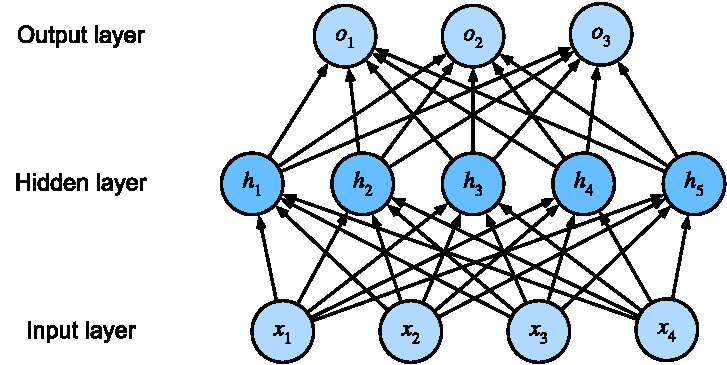
\includegraphics[scale=0.9]{chapters/assets/mlp.pdf}
%     \caption{An MLP with hidden layer consisting of $5$ hidden units. Image courtesy of \textcite{zhang2021dive}.}
%     \label{fig:mlp}
% \end{figure}
\def\layersep{2.5cm}
\begin{figure}
    \centering
    \captionsetup{justification=centering}
    \begin{tikzpicture}[shorten >=1pt,->,draw=black!50, node distance=\layersep]
    \tikzstyle{every pin edge}=[<-,shorten <=1pt]
    \tikzstyle{neuron}=[circle,fill=black!25,minimum size=17pt,inner sep=0pt]
    \tikzstyle{input neuron}=[neuron, fill=tudelft-green!50];
    \tikzstyle{output neuron}=[neuron, fill=tudelft-fuchsia!40];
    \tikzstyle{hidden neuron}=[neuron, fill=tudelft-cyan!50];
    \tikzstyle{annot} = [text width=4em, text centered]

    % Draw the input layer nodes
    \foreach \name / \y in {1,...,4}
    % This is the same as writing \foreach \name / \y in {1/1,2/2,3/3,4/4}
        \node[input neuron, pin=left:Input \#\y] (I-\name) at (0,-\y) {\(\symbfit{x}_{\y}\)};

    % Draw the hidden layer nodes
    \foreach \name / \y in {1,...,5}
        \path[yshift=0.5cm]
            node[hidden neuron] (H-\name) at (\layersep,-\y cm) {\(\symbfit{h}_{\y}\)};

    % Draw the output layer node
    \node[output neuron,pin={[pin edge={->}]right:Output}, right of=H-3] (O-0) {\(\symbfit{o}_{1}\)};
    \node[output neuron,pin={[pin edge={->}]right:Output}, right of=H-2] (O-1) {\(\symbfit{o}_{2}\)};
    \node[output neuron,pin={[pin edge={->}]right:Output}, right of=H-4] (O-2) {\(\symbfit{o}_{3}\)};

    % Connect every node in the input layer with every node in the
    % hidden layer.
    \foreach \source in {1,...,4}
        \foreach \dest in {1,...,5}
            \path (I-\source) edge (H-\dest);

    % Connect every node in the hidden layer with the output layer
    \foreach \source in {1,...,5}
        \foreach \dest in {0,...,2}
            \path (H-\source) edge (O-\dest);

    % Annotate the layers
    \node[annot,above of=H-1, node distance=1cm] (hl) {Hidden layer};
    \node[annot,left of=hl] {Input layer};
    \node[annot,right of=hl] {Output layer};
\end{tikzpicture}
    \caption{An MLP with a hidden layer consisting of $5$ hidden units.}
    \label{fig:mlp}
\end{figure}

Feedforward neural networks are called \textit{networks} because they are typically composed of many different functions. The model is associated with a directed acyclic graph that describes how the functions are composed together.
For example, we can have three functions \(f^{(1)}, f^{(2)}\) and $f^{(3)}$ connected in a chain, to form \(f = f^{(1)} \circ f^{(2)} \circ f^{(3)}\). 
Chain structures such as these are quite commonly used structures of neural networks. Here, $f^{(1)}$ is the \textbf{first layer}, $f^{(2)}$ is the \textbf{second layer} and so on. 
The final layer is called \textbf{output layer}, in this small example, $f^{(3)}$ is the output layer. The training data and training strategy determine what the output layer must produce for each given input $\symbfit{x}$.
Intermediate layers such as $f^{(2)}$ that do not directly produce the output $\symbfit{y}$ are called \textbf{hidden layers}.

Each hidden layer of the network is typically vector valued. The dimensionality of these hidden layers determines \textbf{width} of the model. Each element in the vector plays a role analogous to a neuron. Instead of thinking of a layer as a vector-to-vector function, we can also think of the layer as consisting of many \textbf{units} that act in parallel \parencite{Pinker1988}, each representing a vector-to-scalar function. 
\Cref{fig:mlp} shows a small MLP with a single hidden layer. Each of the nodes in \cref{fig:mlp} represents a value in a vector; this implies that the input $\symbfit{x}$ has a dimensionality of $4$, the hidden layer (intermediate values) has a dimensionality of $5$ and the output has a dimensionality of $3$.

Now, we must choose the form of our model, $f(\symbfit{x} \mathsemicolon \symbfit{\theta})$. Let us choose a linear model parameterised by $\symbfit{\theta}$ consisting of $\symbfit{w}$ and $b$, where $\symbfit{w}$ provides the \textbf{weights} and $b$ provides the \textbf{biases} (or intercepts):
\begin{equation}
    \label{eqn:linear-model}
    f(\symbfit{x}; \symbfit{\theta}) = f(\symbfit{x} ; \symbfit{w}, b)=\symbfit{x}^{\top} \symbfit{w} + b.
\end{equation}

For the model in \cref{fig:mlp} whose hidden layer has $\symbfit{h}$ units, which are calculated by a function \(f^{(1)}(\symbfit{x}; \symbfit{W}, \symbfit{c})\) that is linear similar to the form of \cref{eqn:linear-model}. 
The values of these hidden units are then used as input to the second layer, which is also the output layer of the network. The output layer is also a linear function applied to $\symbfit{h}$ rather than to $\symbfit{x}$.
The network now has two functions chained together \(\symbfit{h} = f^{(1)}(\symbfit{x}; \symbfit{W}, \symbfit{c})\) and \(y = f(\symbfit{h} ; \symbfit{w}, b)\), with the complete model being $f(\symbfit{x} ; \symbfit{W}, \symbfit{c}, \symbfit{w}, b)=f^{(2)}\left(f^{(1)}(\symbfit{x})\right)$. It should be noted that a model parameterised by $\symbfit{\theta}$ implies that $\symbfit{\theta}$ is a collection of all the weights and biases present in the network.

Unfortunately, the complete model $f$ is a linear function of its input, since we have chosen both $f^{(1)}$ and $f^{(2)}$ to be linear. 
However, not all data spaces are linear. More often than not, they are non-linear in nature; accordingly, we must introduce a non-linear function to describe the data and its features.
Most neural networks do so using an \textbf{affine transformation} controlled by the learned parameters (such as $\symbfit{\theta}$), followed by a fixed nonlinear function called an \textbf{activation function}.

\section{Activation Functions} \label{sec:activation-functions}

Activation functions decide whether or not a neuron (node in \cref{fig:mlp}) should be activated. More specifically, they are differentiable operators to transform inputs to outputs and add some form of non-linearity in the transformation. Formally, our hidden-layer output is now defined as:
% \begin{equation}
%     f(\symbfit{x}; \symbfit{\theta}) = f(\symbfit{x}; \symbfit{w}, b) = g(\symbfit{x}^\top\symbfit{w} + b)
% \end{equation}
\begin{equation}
\begin{split}
    \symbfit{h} &= g \circ f^{(1)} \left(\symbfit{x}\right)\\
                &=g\left(\symbfit{W}^{\top} \symbfit{x}+\symbfit{c}\right)
\end{split}
\end{equation}
where $\symbfit{W}$ is the linear transformation, $\symbfit{c}$ the biases and $g(\cdot)$ is an \textbf{activation function} whose job is to introduce some non-linearity. Previously, we had used a vector of weights and a scalar bias parameter in \cref{eqn:linear-model} to describe an affine transformation from a vector input to a scalar output. However, now we are describing an affine transformation from a vector $\symbfit{x}$ to a vector $\symbfit{h}$, so an entire vector of biases is needed.

One of the most widely used activation functions is \textbf{ReLU} (Rectified Linear Unit) \parencite{Fukushima1975}. This function simply returns the maximum between the given input value and zero, as given in \cref{eqn:relu}. As such, this simple function has a minimal computation cost and can be performed quite quickly.
\begin{equation}\label{eqn:relu}
    \begin{split}
        g \circ f(\symbfit{x}) & = \operatorname{max}\left(0, f^{(1)}(\symbfit{x})\right)\\
                               & = \operatorname{max}\left(0, \symbfit{W}^\top\symbfit{x} + \symbfit{c}\right)
    \end{split}
\end{equation}

Another important and common function is the \textbf{Sigmoid} \cref{eqn:sigmoid} function. This function maps the input value to a real number between $(0, 1)$.
In earlier forms of nerural networks \parencite{mcculloch1943logical}, scientists where interested in neurons that either fire or do not, and so used thresholding units. A thresholding activation takes value $0$ when its input is below a certain threshold and takes value $1$ if its input is higher than the threshold. 
Sigmoids, on the other hand, are smooth and differentiable approximations of thresholding units; this is favourable to the gradient-based learning adopted in today's time.
Sigmoids are used largely in output units when we want to interpret the output as probabilities for binary classification problems.
\begin{equation}\label{eqn:sigmoid}
    \begin{split}
        \operatorname{sigmoid}(\symbfit{x}) = \sigma(\symbfit{x}) & = \frac{1}{1 + \exp(-\symbfit{x})}.
        % \operatorname{sigmoid}(\symbfit{h}) & = \frac{1}{1 + \exp(-(\symbfit{W}^\top\symbfit{x}+\symbfit{c}))}.
    \end{split}
\end{equation}

Like the sigmoid function, the \textbf{tanh} (hyperbolic tan) function also squashes its inputs, mapping them between $-1$ and $1$:
\begin{equation}
\begin{split}
    \operatorname{tanh}(\symbfit{x}) & = \frac{1 - \exp(-2\symbfit{x})}{1 + \exp(-2\symbfit{x})}.
    % \operatorname{tanh}(\symbfit{h}) & = \frac{1 - \exp(-2(\symbfit{W}^\top\symbfit{x}+\symbfit{c}))}{1 + \exp(-2(\symbfit{W}^\top\symbfit{x}+\symbfit{c}))}.
\end{split}
\end{equation}

\begin{figure}[t]
     \centering
     \captionsetup{justification=centering}
     \begin{subfigure}[b]{0.3\textwidth}
         \centering
         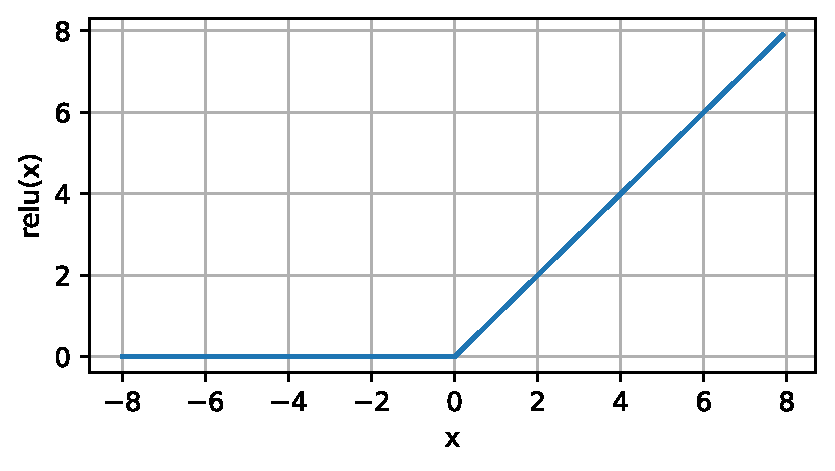
\includegraphics[width=\textwidth]{chapters/assets/relu.pdf}
         \caption{ReLU}
         \label{fig:relu}
     \end{subfigure}
     \hfill
     \begin{subfigure}[b]{0.3\textwidth}
         \centering
         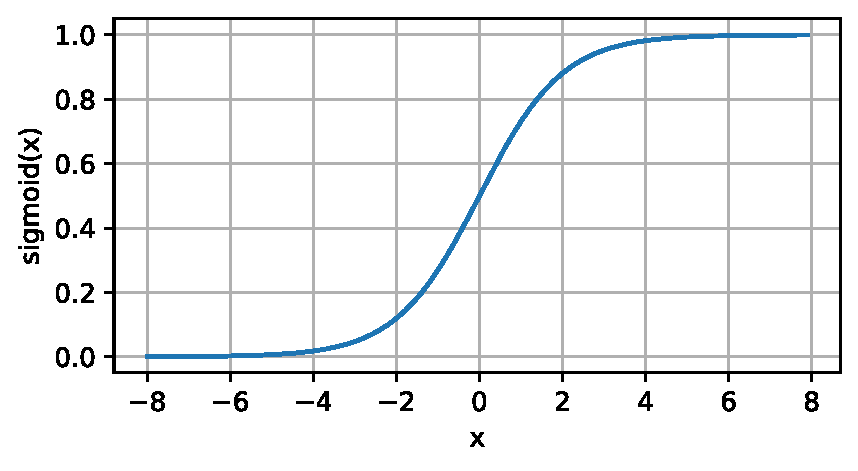
\includegraphics[width=\textwidth]{chapters/assets/sigmoid.pdf}
         \caption{Sigmoid}
         \label{fig:sigmoid}
     \end{subfigure}
     \hfill
     \begin{subfigure}[b]{0.3\textwidth}
         \centering
         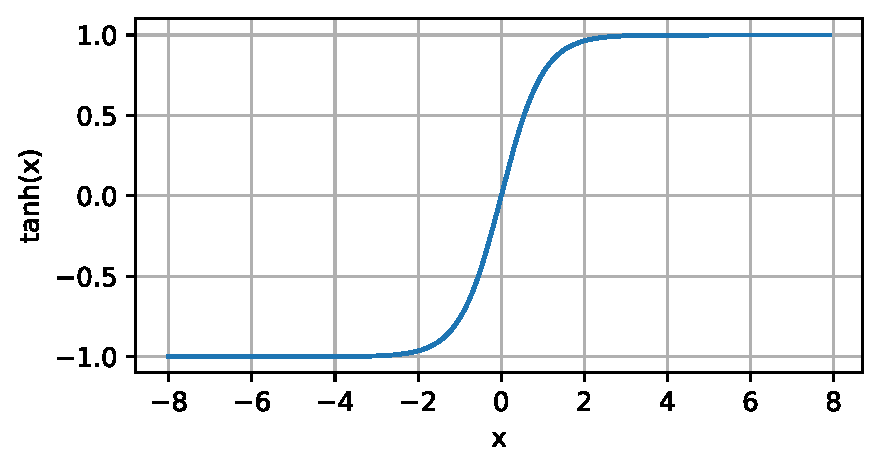
\includegraphics[width=\textwidth]{chapters/assets/tanh.pdf}
         \caption{Tanh}
         \label{fig:tanh}
     \end{subfigure}
        \caption{Three common activation functions.}
        \label{fig:three-activation-funcs}
\end{figure}

\section{Loss Function}\label{sec:loss-fn}
During training, for each training sample in the training set $\{\symbfit{x}_i, y_i\}_{i=1}^N$ where $\symbfit{x}_i$ is an input vector and $y_i$ is the corresponding label, we present the input $\symbfit{x}$ to the neural network and compare the predicted output of the network $\hat{y}_i$ with the corresponding label $y_i$.
We need to define a \textbf{loss function} to objectively measure how much the predicted output of the network $\hat{y}_i$ is different from the expected output $y_i$. For regression problems, the quadratic loss function called the mean squared error (MSE) is calculated as follows:
\begin{equation}
    \mathcal{L}({\hat{y}}, {y}) = \frac{1}{2} \| {y} - {\hat{y}} \| ^ 2
\end{equation}

The loss function is calculated for each training example in the training set. The average of the calculated loss functions for all training examples in the training set is called the \textbf{cost function}. For MSE it is the average of the calculated loss functions for all training examples in the training set:
\begin{equation}
    J(\symbfit{\theta}) = \frac{1}{2N} \sum_{i=1}^{N} \| {y}_i - {\hat{y}_i} \| ^ 2
\end{equation}
where $N$ is the total number of training samples. In the following \Cref{sec:softmax} we shall see another loss function that is important for multiclass classification.

\section{Softmax} \label{sec:softmax}
For convenience in the following section, we shall call the output of network $f(\symbfit{x}; \symbfit{\theta})$ as $\symbfit{o}$. Assume that we have a loss function such as mean squared error loss (MSE). When working with \textbf{multiclass classification} problems, where \(\symbfit{y} \in \left\{1,\ldots, K \right\}\); we expect the output of the model to be a vector of class probabilities where each value tells us the probability that a sample belongs to a particular class.
Note that we generally employ the ``one-hot'' encoding mechanism where $\symbfit{y} = (0, ... , 0, 1, 0, ... , 0)$.
We can try to directly minimise the difference between $\symbfit{o}$ and $\symbfit{y}$. Although treating classification as a regression problem may work well, it still lacks in two main ways:
\begin{itemize}
    \item There is no guarantee that $\symbfit{o}$ will sum up to $1$ as we have come to expect from probabilities
    \item There is no guarantee that $\symbfit{o}$ takes strictly non-negative values regardless of the sum of $\symbfit{o}$
\end{itemize}

Both of these issues make the problem difficult to solve in addition to making the solution highly sensitive to outliers. If we were to presume a positive linear dependency between the horsepower of a car and the probability that someone will buy it, the probability might exceed $1$ when it comes to buying a Bugatti Chiron\footnote{\url{https://www.bugatti.com/models/chiron-models/}}! Of course, this breaks the mathematical and logical rules of probability theory; therefore, we need a technique to map the values of $\symbfit{o}$ between $(0, 1)$.
% TODO: should we talk about data generating distribution here?

One way to accomplish these goals (ensuring that the output sums up to $1$ and its values are non-negative), is to use an exponential function $P(y = i) \propto \exp o_i$. The $\exp$ function does ensure that the output will always be non-negative. We can further \textbf{normalise} these values so that they add up to $1$ by dividing each by the sum of the whole. This gives us the \textbf{softmax} function:
\begin{equation}
    \hat{\symbfit{y}} = \operatorname{softmax}(\symbfit{o}) \quad \text{where}\quad \hat{y}_i = \frac{\exp(o_i)}{\sum_{j=1}^{K} \exp(o_j)}.
    \label{eqn:std-softmax}
\end{equation}

Note that the highest value in $\symbfit{o}$ corresponds to the most likely class according to $\symbfit{\hat{y}}$. Softmax also preserves the ordering of its arguments as shown in the example:
\begin{equation}
    \nonumber
    \operatorname{softmax} \left(\begin{bmatrix}
    8\\
    5\\
    0
    \end{bmatrix}\right)
    = 
    \begin{bmatrix}
    0.9523\\
    0.0474\\
    0
    \end{bmatrix}.
\end{equation}

\subsection{Softmax and Cross-Entropy Loss}\label{ssec:ce-loss}

The softmax function gives us a vector $\symbfit{\hat{y}}$, which we can interpret as (estimated) conditional probabilities of each class, given any input $\symbfit{x}$, like $P(y=\text{class} | \symbfit{x})$. 
The cross-entropy loss measures the difference between two probability distributions; in this case, it measures the difference between $\symbfit{\hat{y}}$ and $\symbfit{y}$. The cross-entropy loss is given as:
\begin{equation}\label{eqn:ce-loss}
    \mathcal{L}(\symbfit{y}, \hat{\symbfit{y}}) = - \sum_{j=1}^K \symbfit{y}_j \log \hat{\symbfit{y}}_j.
\end{equation}

Note that the loss defined in \cref{eqn:ce-loss}, has a lower bound of $0$ when $\hat{\symbfit{y}}$ is a probability vector, that is, no single entry is greater than $1$, and hence its negative logarithm cannot be lower than $0$. For multiclass classification problems, the cost function is calculated as follows:
\begin{equation}
    J(\symbfit{\theta}) = - \frac{1}{N} \sum_{j=1}^{N} \sum_{i=1}^{K} \symbfit{y_{i}^{(j)}}\log(\symbfit{\hat{y}_{i}^{(j)}})
\end{equation}
where $\symbfit{y_{i}^{(j)}}$ and $\symbfit{\hat{y}_{i}^{(j)}}$ are the true and predicted output for the $j\textsuperscript{th}$ input sample $\symbfit{x}_j$. To better understand the origins of the cross-entropy loss, please refer to \textcite{zhang2021dive}.

\subsection{Softmax vs Sigmoid}\label{ssec:softmax-vs-sigmoid}
The softmax and sigmoid functions are similar, as they help squeeze the network output within a certain range. The softmax function operates on a vector input, while the sigmoid takes a scalar value as input. In fact, the sigmoid function is a special case of the softmax function for a classifier with only two input classes (binary classification problem). We can show this if we set the input vector to $\symbfit{z} = [x, 0]$ and calculate the first output element with the usual softmax formula:
\begin{align*}
    \operatorname{softmax}(\symbfit{z})_{1}&=\frac{\exp{(z_{1})}}{\exp{(z_{1})}+\exp(z_{2})} \\
    &= \frac{\exp(x)}{\exp(x)+\exp(0)} \\
    &= \frac{\exp(x)}{\exp(x)+1} && \text{divide numerator and denominator by} \exp{(x)}\\
    &= \frac{1}{1 + \exp(-x)}
\end{align*}


\section{Universal Approximation Theory}\label{sec:uat}

MLPs are of extreme importance in deep learning, as they form the basis for many applications and advanced neural architectures. To do this, MLPs and neural networks, in general, must be able to approximate a wide range of functions, given enough input data to learn from. Neural networks started as a way to mimic the neural structure of the brain \parencite{mcculloch1943logical}, and as we know our brain is capable of complex statistical analysis, among other things. As such, a worthwhile question to ask here is \textit{just how powerful can a deep neural network be?}
Fortunately for us, this question has been answered several times in the context of MLPs and radial basis functions (RBF) \parencite{Cybenko1989, Micchelli1986, Hornik1991}. These works suggest that even with a single hidden layer, given enough nodes and the right set of parameters $\symbfit{\theta}$, we can potentially model any function. 
In simple terms, having enough nodes and stacking enough affine transformations followed by non-linear transforms repetitively, a neural network should be able to model a highly rich class of functions.
Although neural networks are capable of expressing arbitrary continuous functions, it may not be easy to learn the function and its parameters.

\section{Optimisation and Backpropagation}\label{sec:optimisation}

Until now, we have only discussed the forward pass of a neural network, where the network processes the input $\symbfit{x}$. However, to effectively approximate $f^\star$, a neural network must learn an ideal set of values for the parameters, $\symbfit{\theta}$. To do so, we must \textbf{optimise} the weights so that they are suitable for the task and the data at hand. However, the optimisation algorithms used to train deep learning models differ from traditional optimisation algorithms in multiple ways. In most machine tasks, we are concerned with some performance measure $P$, which is defined with respect to the test set and may very well be intractable. Therefore, we optimise $P$ indirectly through a cost function $J\symbfit{(\theta)}$.

Typically, the cost function is written as an average over the training set (see \Cref{sec:loss-fn}):
\begin{equation}
\label{eqn:cost-fn-emp}
\begin{split}
    J(\symbfit{\theta})&=\mathbb{E}_{(\symbfit{x}, \mathrm{y}) \sim \hat{p}_{\mathrm{data}}} \mathcal{L}(f(\symbfit{x} ; \symbfit{\theta}), y)\\
    &= \mathbb{E}_{(\symbfit{x}, \mathrm{y}) \sim \hat{p}_{\mathrm{data}}} \mathcal{L}(\hat{y}, y)
\end{split}
\end{equation}
where $\mathcal L$ is the loss function per sample, $\hat{y} = f(\symbfit{x}; \symbfit{\theta})$ is the predicted output, the input is $\symbfit{x}$ and \(\hat{p}_{\mathrm{data}}\) is the empirical (observed) distribution. In the straightforward supervised case, $y$ is the true target output. It takes minimal effort to adapt this formulation to exclude $y$ as an argument, as we shall see this in \Cref{chap:self-supervised-learning}.


\subsection{Gradient Descent}\label{sec:sgd}

We begin by assuming that we have a function $y = f(x)$ where $x, y \in \mathbb{R}$ and that it has a derivative $f^\prime(x)$. The derivative of a function gives its slope, also called \textbf{gradient} at a certain input point $x$. The gradient indicates how adding a small change $\epsilon$ to $x$ will affect the output: $f(x + \epsilon) \approx f(x) + \epsilon f^\prime(x)$. Gradient descent is a first-order iterative optimisation algorithm used to find the local minimum or maximum of a function \parencite{Kiefer1952, Robbins1951}. The optimisation algorithm works by iteratively moving in the direction of steepest descent, as defined by the negative of the gradient.

\begin{figure}[ht]
    \centering
    \captionsetup{justification=RaggedRight}
    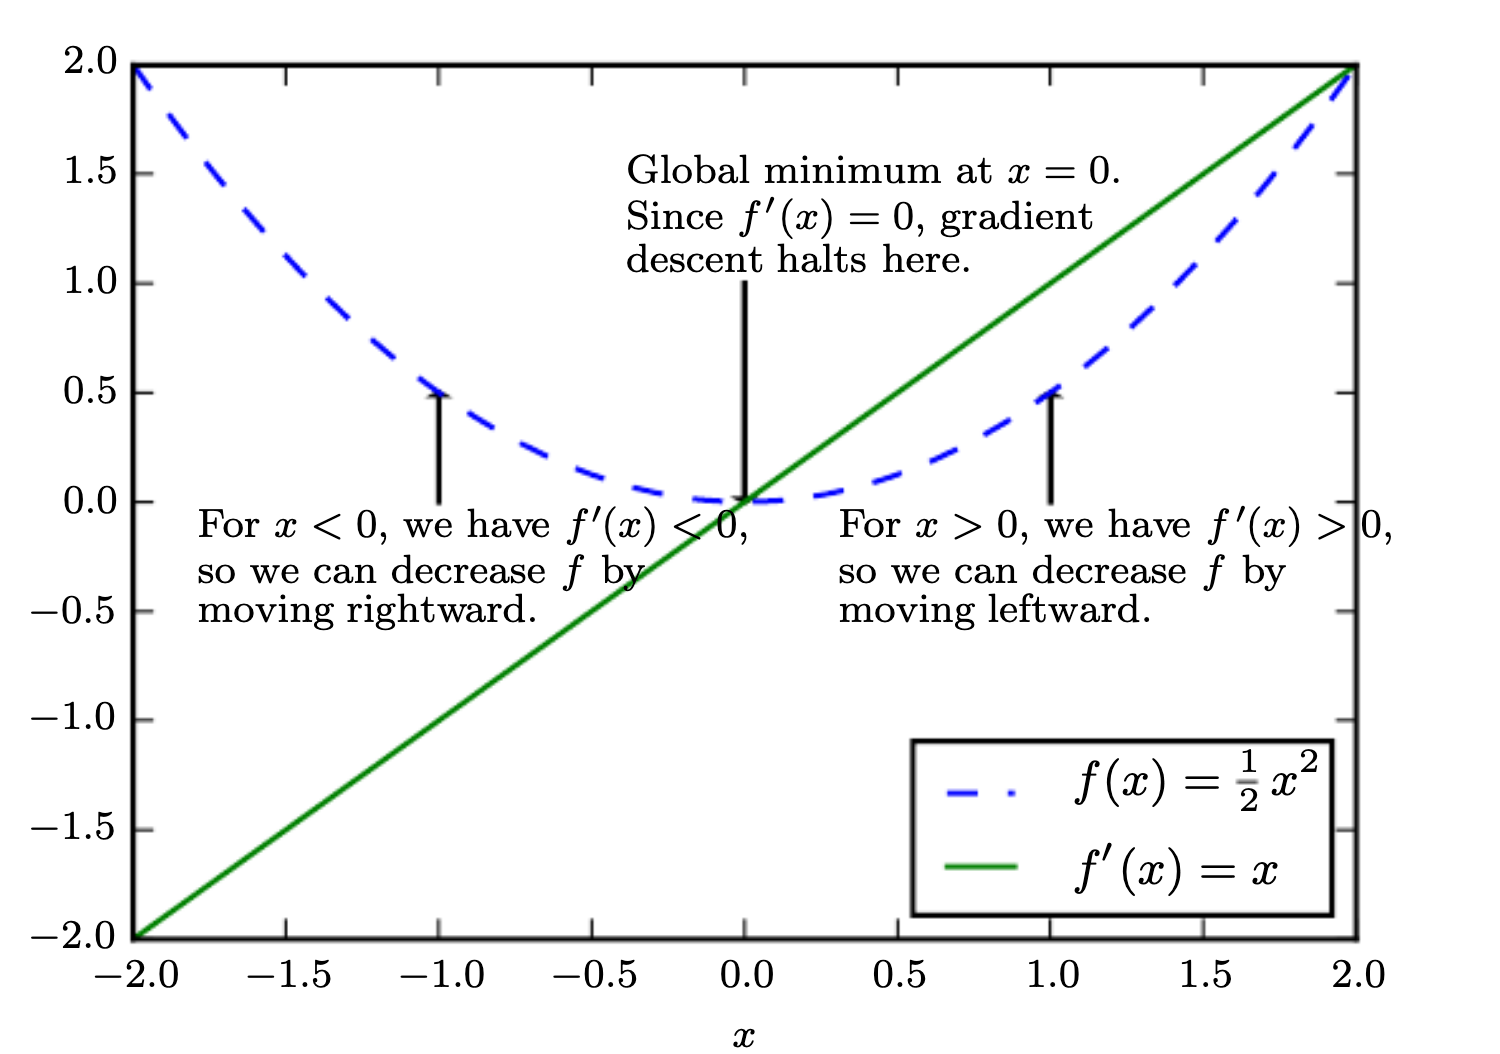
\includegraphics[scale=0.15]{chapters/assets/gradient_descent_basic.png}
    \caption{Gradient descent algorithm illustration for finding the minimum of a function $f(x) = \frac{1}{2}x^2$. Beginning with either positive of negative values of $x$, the gradient descent algorithm will find a minima at $x=0$ by moving in the direction opposite the sign of the gradient given by $f^\prime(x)=x$. Figure courtesy of \textcite{GoodfellowDLBook2016}.}
    \label{fig:gradient-descent}
\end{figure}

In \cref{fig:gradient-descent} the function $f(x)=\frac{1}{2}x^2$ depends only on the input $x$ and has a derivative \(f^\prime(x)=x\). In order to find the minimum of $f(x)$ we must find the value of $x$ where $f^\prime(x)=0$. The useful property of the gradient is that it tells us how to change $x$ to make a small change to $y$. For instance, we can infer that $f\left(x-\epsilon \operatorname{sign}\left(f^{\prime}(x)\right)\right) \ll f(x)$ for a small $\epsilon$. 
Therefore, to reduce $f(x)$, we can begin this process by starting with positive or negative values of $x$ and moving in the direction opposite to the sign of the gradient $f^\prime(x)$. The process is known as \textbf{gradient descent}, more specifically this update step reads:
\begin{align}
    x^\prime &=x-\epsilon \operatorname{sign}\left(f^{\prime}(x)\right) \nonumber \\
    &= x-\epsilon \operatorname{sign}\nabla_x f(x) \quad
\end{align}

\subsection{Backpropagation}\label{eqn:backprop}
The backpropagation as a learning algorithm was put forth by \textcite{rumelhart1986learning}, and is firmly based on the concept of gradient descent. We discussed gradient descent in the context of a simple function $f(x)$ that was dependent only on its input $x$, however, neural networks depend on the input $\symbfit{x}$ and a set of parameters $\symbfit{\theta}$, $f(\symbfit{x} \mathsemicolon \symbfit{\theta})$. Furthermore, the learning goal of neural networks is not to directly minimise the function $f(\symbfit{x} \mathsemicolon \symbfit{\theta})$. Rather, the goal of learning in neural networks is to minimise the cost function (or loss function) given the training set. 

Consider a network parameterised by $\symbfit{\theta} = \{\symbfit{w}, b\}$. The goal of backpropagation is to calculate partial derivatives \(\sfrac{\partial J}{\partial \symbfit{w}}\) and \(\sfrac{\partial J}{\partial b}\) of the cost function $J$ with respect to weight $\symbfit{w}$ and bias $b$. To further concretize the notion, we shall use the MSE loss from \Cref{sec:loss-fn}:
\begin{align}
    \mathcal{L}(\symbfit{\hat{y}}, \symbfit{y}) &= \frac{1}{2} \| \symbfit{y} - \symbfit{\hat{y}} \| ^ 2 \\
    J(\symbfit{\theta}) &= \frac{1}{2N} \sum_{i=1}^{N} \mathcal{L}(f(\symbfit{x} \mathsemicolon \symbfit{\theta}), \symbfit{y})
    \label{eqn:bp-cost-fn}
\end{align}
where $N$ is the total number of training samples. To calculate \(\sfrac{\partial J}{\partial \symbfit{w}}\) and \(\sfrac{\partial J}{\partial b}\), we apply the \textbf{chain rule} and calculate, in turn, the gradient of each intermediate variable and parameter. The first step is to calculate $\sfrac{\partial J}{\partial \mathcal{L}}$ which are the gradients of the cost function in \Cref{eqn:bp-cost-fn} with respect to the loss term $\mathcal{L}$.
Next, we must compute the gradient of the cost function with respect to the output variable $\symbfit{\hat{y}}$ according to the chain rule:
\begin{equation}
    \frac{\partial J}{\partial \symbfit{\hat{y}}}
= \frac{\partial J}{\partial \mathcal{L}} \times \frac{\partial \mathcal{L}}{\partial \symbfit{\hat{y}}}.
\end{equation}
Now we can calculate the gradient \(\sfrac{\partial J}{\partial \symbfit{w}}\), using the chain rule this yields:
\begin{equation}
    \frac{\partial J}{\partial \symbfit{w}}= \left(\frac{\partial J}{\partial \symbfit{\hat{y}}} \times \frac{\partial \symbfit{\hat{y}}}{\partial \symbfit{w}}\right).
\end{equation}
where \(\sfrac{\partial \symbfit{\hat{y}}}{\partial \symbfit{w}} = \symbfit{x}\).
Notice that the order of calculations are now \textbf{reversed} relative to those performed in the forward pass. Here we start with the output emitted by the neural network and work our way backwards towards the parameters. We can repeat the above steps for computing \(\sfrac{\partial J}{\partial b}\). Intuitively, this tells us how to update $\symbfit{w}$ and $b$ in order to reduce $J(\symbfit{\theta})$.

We must also be aware of the fact that we optimise for the loss function $\mathcal{L}$, that is, we are trying to find the optimal set of parameters $\symbfit{\theta}$ that will give us the lowest value of the loss function across $N$ training samples. In other words, we are trying to find the minima of $\mathcal L$ with respect to the input $\symbfit x$ and the parameters $\symbfit{\theta}$.
The gradient $\nabla_{\symbfit{\theta}}J$ across all samples is given as:
\begin{equation}
    \nabla_{\theta} J(\symbfit{\theta}) = \frac{1}{2N} \sum_{i=1}^{N}\nabla_{\symbfit{\theta}}\mathcal{L}(f(\symbfit{x};\symbfit{\theta}), y)
    % \bigg[\frac{\partial L}{\partial w}, \frac{\partial L}{\partial b}, \ldots \bigg]^\top
\end{equation}
where $\nabla_{\theta} J(\symbfit{\theta})$ is the average of the gradients of the loss function with respect to $\symbfit x$ and $\symbfit{\theta}$. The parameter update using the gradient descent algorithm with step size $\eta$ can be written as
\begin{equation}
    \label{eqn:basic-gd}
    \symbfit{\theta}^\prime=\symbfit{\theta}-\eta \nabla_{\theta} J(\symbfit{\theta}).
\end{equation}

However, this method is intractable for very large values of $N$. Therefore, we choose to compute gradients for a smaller set of $m$ samples such that $m \ll N$:
\begin{equation}
\label{eqn:sgd-proper}
    \nabla_{\theta} J(\symbfit{\theta}) = \frac{1}{2m} \sum_{i=1}^{m}\nabla_{\symbfit{\theta}}\mathcal{L}(f(\symbfit{x};\symbfit{\theta}), y).
    % \bigg[\frac{\partial L}{\partial w}, \frac{\partial L}{\partial b}, \ldots \bigg]^\top
\end{equation}
This is the idea of stochastic approximation behind \textbf{stochastic gradient descent} (SGD). It is an approximation of the gradient from a small number of input samples \parencite{Bottou2016}. The SGD update step in \cref{eqn:sgd-proper} is similar to \Cref{eqn:basic-gd}.
% \begin{equation}
% \symbfit{\theta}^{\prime}=\symbfit{\theta}-\eta \frac{1}{2m} \sum_{i=1}^{m} \nabla_{\symbfit{\theta}}J(\symbfit{\theta}).
% \end{equation}

Finally, for a network with $l$ layers, there are just as many gradients with respect to the loss function $\mathcal{L}$:
\begin{equation}
    \symbfit{\nabla_{\theta}} \mathcal{L}(f(\symbfit{x};\symbfit{\theta}), y) = \bigg[\frac{\partial \mathcal{L}}{\partial w^{(l)}}, \frac{\partial \mathcal{L}}{\partial b^{(l)}}, \frac{\partial L}{\partial w^{(l-1)}}, \frac{\partial \mathcal{L}}{\partial b^{(l-1)}}, \ldots, \frac{\partial \mathcal{L}}{\partial w^{(1)}}, \frac{\partial \mathcal{L}}{\partial b^{(1)}}\bigg]^\top
\end{equation}
where $\symbfit{\nabla_{\theta}} L(f(\symbfit{x};\symbfit{\theta}), y)$ is a vector of partial derivatives with respect to the weights in the neural network model while $w^{(l)}$ and $b^{(l)}$ are the weights and biases of layer $l$.

\import{chapters/}{02_basics_of_dl}

\chapter{Related Work} \label{chap:related-work}




%% Use letters for the chapter numbers of the appendices.
\appendix

%\input{appendix-a}

\printbibliography

\end{document}

